% works on TeX-Live 2015

\documentclass{beamer}
\usepackage{tgheros}
\usepackage[varqu, scaled=1.1]{inconsolata}
%\usepackage{mylistings}
\usepackage{csquotes}
\usepackage{hyperref}
\usepackage{xcolor}
\usepackage{graphicx}
\usepackage{siunitx}
\usepackage{booktabs}
%\usepackage{tikz}
%\usepackage{tikz-uml}

% \lstset{
%   style=colored,
%   %belowskip=0pt
%   basicstyle=\ttfamily\small\color{darkgray},
%   columns=[c]fixed,
%   gobble=4
% }

% colors
\providecolor{textgreen}{RGB}{59, 158, 72}
\providecolor{textblue}{RGB}{15, 100, 255}
\providecolor{textred}{RGB}{255, 51, 66}

\usetheme[compress]{Singapore}
\useinnertheme{circles}
\setbeamercolor{structure}{fg=textblue}
%\setbeamercolor{block body alerted}{bg=normal text.bg!90!black}
\setbeamercolor{block body}{bg=normal text.bg!90!black}
%\setbeamercolor{block body example}{bg=normal text.bg!90!black}
%\setbeamercolor{block title alerted}{use={normal text,alerted text},fg=alerted text.fg!75!normal text.fg,bg=normal text.bg!75!black}
\setbeamercolor{block title}{fg=black, bg=textblue!90}
%\setbeamercolor{block title example}{use={normal text,example text},fg=example text.fg!75!normal text.fg,bg=normal text.bg!75!black}

% smaller footnotes; see: http://tex.stackexchange.com/a/192652/46356
\setbeamertemplate{footnote}{%
  \tiny%
  \parindent 1em\noindent%
  \raggedright
  \hbox to 1.8em{\hfil\insertfootnotemark}\insertfootnotetext\par%
}%
\setlength\footnotesep{0pt}

\author{Philipp Gabler}
\title{Project 2}
\date{2017-02-03}

%%%%%%%%%%%%%%%%%%%%%%%%%%%%%%%%%%%%%%%%%%%%%%%%%%%%%%%%%%%%%%%%%%%%%%%%%%%%%%%%%%%%%%%%%%%%%%%%%%%%
\begin{document}
\beamertemplatenavigationsymbolsempty

\section{Motivation}
\begin{frame}{Fast percolation}
  \begin{block}{Reminder}
    Percolation is the study of the global connection behaviour of a network when removin a certain
    fraction of its nodes, measured in the (relative) size of the larges connected component.
  \end{block}
  
  \begin{itemize}
  \item Goal: learn a way of informed percolation which optimally disconnects a network (remove
    minimum amount of nodes with maximum effect)
  \item Useful for preventing desease spreading, or to find critical nodes in the network
  \end{itemize}
\end{frame}


%%%%%%%%%%%%%%%%%%%%%%%%%%%%%%%%%%%%%%%%%%%%%%%%%%%%%%%%%%%%%%%%%%%%%%%%%%%%%%%%%%%%%%%%%%%%%%%%%%%%
\section{Methodology}
\begin{frame}{Setting up a model}
We attach to each node a Bernoulli random variable of failure:
\begin{align*}
  \hat{\mathbf{p}}_i &= \sigma(\mathbf{w}^T \cdot \mathbf{info}_i) \\
  \mathbf{Fail}_i(\varphi) &\sim \text{Bernoulli}\left(\hat{\mathbf{p}}_i\,
                      \frac{\varphi}{\frac{1}{n}\sum_i \hat{\mathbf{p}}_i}\right)
\end{align*}
where \(\sigma\) is the logistic function, \(\mathbf{info}\) is a vector of local information (eg.,
degree), and \(\mathbf{w}\) the weighting of this information (a logistic model, sort of).

The value \(\varphi\) varies in \([0; 1]\) and describes the expected fraction of failing nodes.  The
individual probabilities are scaled accordingly.
\end{frame}



%%%%%%%%%%%%%%%%%%%%%%%%%%%%%%%%%%%%%%%%%%%%%%%%%%%%%%%%%%%%%%%%%%%%%%%%%%%%%%%%%%%%%%%%%%%%%%%%%%%%
\section{Experimental Setup}
\begin{frame}
  \begin{itemize}
  \item Minimize the area under the percolation curve with respect to the weights \(\mathbf{w}\)
  \item This involves sampling the curves (several times) at each parameter evaluation
  \item This is expensive, so I used simulated annealing~-- it requires the least amount of
    evaluations of the loss function
  \item Compare some different network types:
  \end{itemize}

  \begin{center}
    \begin{tabular}{lrrrrrr}
      \toprule
      & \multicolumn{2}{c}{Facebook} & \multicolumn{2}{c}{Traffic} & \multicolumn{2}{c}{Random} \\
      & Train & Test & Train & Test & Train & Test \\
      \midrule
      Vertices & 572 & 347 & 7388 & 13389 & 2000 & 2000\\
      Edges & 3192 & 2519 & 10591 & 21246 & 5000 & 5000\\
      Density & 0.0195 & 0.0419 & 0.0004 & 0.0002 & \multicolumn{2}{c}{\(\approx\) 0.0025}\\
      \bottomrule
    \end{tabular}
  \end{center}
\end{frame}



%%%%%%%%%%%%%%%%%%%%%%%%%%%%%%%%%%%%%%%%%%%%%%%%%%%%%%%%%%%%%%%%%%%%%%%%%%%%%%%%%%%%%%%%%%%%%%%%%%%%
\section{Results}
\begin{frame}

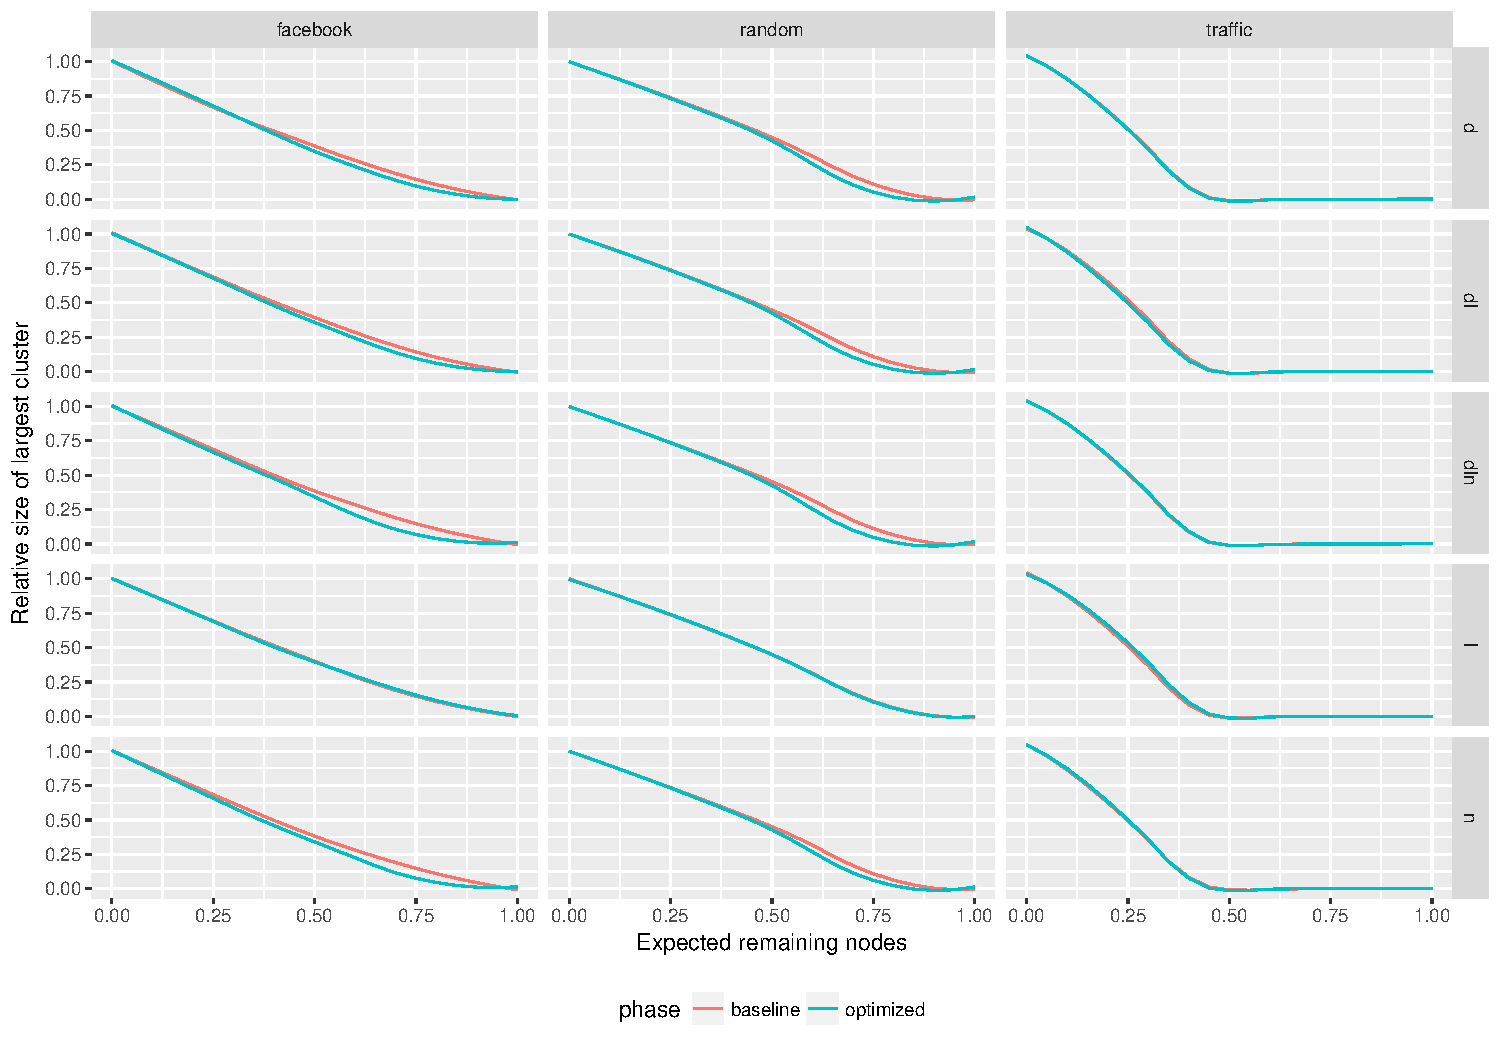
\includegraphics[width=\textwidth]{results.pdf}
  
  % (facebook, d): [0.5] 0.3283630364889754
  % (traffic, d): [0.65] 0.21074304493798848
  % (random, d): [0.25] 0.4201843461802456
  % (facebook, i): [-1.1] 0.1810805834740875
  % (traffic, i): [0.25] 0.2216547318219854
  % (random, i): [0.4] 0.4517175677606427
  % (facebook, l): [1.1] 0.4122167795684476
  % (traffic, l): [0.2] 0.21651320595420895
  % (random, l): [0.2] 0.4409616979378643
  % (facebook, n): [0.05] 0.3342488376071866
  % (traffic, n): [0.5] 0.21555049861067138
  % (random, n): [0.05] 0.42808389546611614
  % (facebook, dl): [0.400757,0.737475] 0.3283141710201117
  % (traffic, dl): [0.188876,-0.214628] 0.21135127079299312
  % (random, dl): [0.301184,-0.765181] 0.4183382696586946
  % (facebook, dln): [0.185994,-0.475402,0.0138872] 0.3297293375203304
  % (traffic, dln): [0.194423,0.255597,0.73907] 0.217658817732126
  % (random, dln): [0.147955,-0.133006,0.0134066] 0.423664340534555

  % (facebook, d): [-0.55] 0.471840848722235
  % (traffic, d): [-0.6] 0.21650355502500723
  % (random, d): [-0.1] 0.44100544039781314
  % (facebook, i): [-0.35] 0.18307828314919564
  % (traffic, i): [0.35] 0.21951807775693943
  % (random, i): [-0.2] 0.43784038404490977
  % (facebook, l): [2.3] 0.38007060763692424
  % (traffic, l): [-0.25] 0.21509237602182799
  % (random, l): [0.05] 0.44265720078375076
  % (facebook, n): [0.2] 0.4689802470340089
  % (traffic, n): [-0.25] 0.21884265918897558
  % (random, n): [-0.4] 0.44351458013359263
  % (facebook, dl): [-0.676532,1.5025] 0.4023356042400362
  % (traffic, dl): [0.233561,-0.0764628] 0.2179749210675988
  % (random, dl): [-0.00159558,-0.0980889] 0.4421562417761069
  % (facebook, dln): [-0.0484588,1.15782,-0.069973] 0.406014520990275
  % (traffic, dln): [0.0800902,0.150924,0.0781754] 0.21748833595083378
  % (random, dln): [0.506437,0.120634,0.286868] 0.4413333259116106
  
\end{frame}



%%%%%%%%%%%%%%%%%%%%%%%%%%%%%%%%%%%%%%%%%%%%%%%%%%%%%%%%%%%%%%%%%%%%%%%%%%%%%%%%%%%%%%%%%%%%%%%%%%%%
\section{Discussion}
\begin{frame}
  
\end{frame}


% @misc{snapnets,
%   author       = {Jure Leskovec and Andrej Krevl},
%   title        = {{SNAP Datasets}: {Stanford} Large Network Dataset Collection},
%   howpublished = {\url{http://snap.stanford.edu/data}},
%   month        = jun,
%   year         = 2014
% }

\end{document}